\documentclass[border=10pt, tikz]{standalone}
\usepackage{tikz}
\usepackage{fontspec}
\setmainfont{Songti SC}
\setsansfont{Heiti SC}
\usetikzlibrary{arrows.meta, positioning}

\begin{document}
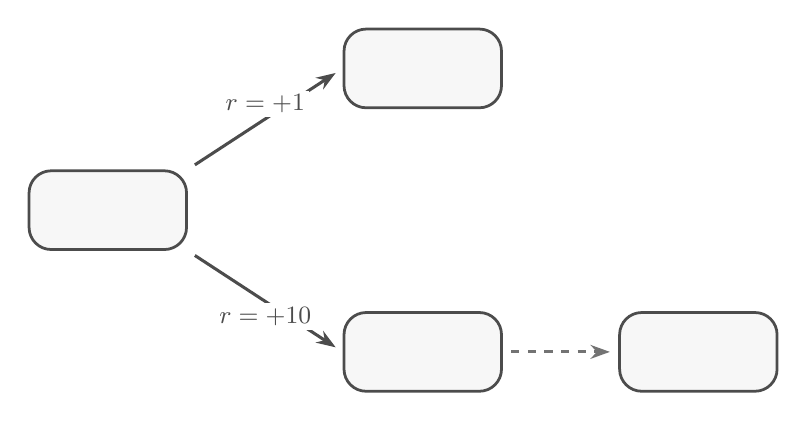
\begin{tikzpicture}[
    box/.style={
        draw=black!70, rounded corners=8pt, minimum width=2.0cm, minimum height=1.0cm,
        font=\normalsize, align=center, line width=1pt, fill=black!3
    },
    arrow/.style={
        -{Stealth[length=7pt, width=5pt]}, line width=1.1pt, black!70,
        shorten >=3pt, shorten <=3pt
    },
    dashedarrow/.style={
        -{Stealth[length=7pt, width=5pt]}, line width=1.1pt, black!55, dashed,
        shorten >=3pt, shorten <=3pt
    },
    lbl/.style={font=\small, text=black!70, fill=white, inner sep=1.5pt}
]

\node[box] (start) at (0, 0) {};
\node[box] (small) at (4.0, 1.8) {};
\node[box] (big) at (4.0, -1.8) {};
\node[box] (danger) at (7.5, -1.8) {};

\draw[arrow] (start.north east) -- node[above, lbl, pos=0.5] {$r=+1$} (small.west);

\draw[arrow] (start.south east) -- node[below, lbl, pos=0.5] {$r=+10$} (big.west);

\draw[dashedarrow] (big.east) -- node[above, lbl, pos=0.5] {} (danger.west);

\end{tikzpicture}
\end{document}
